% !TeX program = lualatex
% Lualatex is important to render Fira fonts; with pdflatex it's just the regular one
\documentclass[12pt]{beamer}


\usepackage{xcolor}

\usetheme{metropolis}
\usepackage{appendixnumberbeamer}

% adjust the background to be completely white
\setbeamercolor{background canvas}{bg=white}

\usepackage{booktabs}
\usepackage[scale=2]{ccicons}

\usepackage{pgfplots}
\usepgfplotslibrary{dateplot}

% typeset mathematics on serif
\usefonttheme[onlymath]{serif}

% better bibliography using biber as backend
\usepackage[natbib=true,backend=biber,style=authoryear-icomp,maxbibnames=30,maxcitenames=16,uniquelist=false,giveninits=true,doi=false,url=true,dashed=false,isbn=false]{biblatex}
% shared bibliogrphy
\addbibresource{../dl4nlp-bibliography.bib}
% disable "ibid" for repeated citations
\boolfalse{citetracker}

% TODOs
\usepackage{todonotes}
\let\todox\todo
\renewcommand\todo[1]{\todox[inline]{#1}}

\definecolor{76abdf}{RGB}{118, 171, 223}

\setbeamercolor{frametitle}{bg=76abdf, fg=white}

\usepackage{xspace}
\newcommand{\themename}{\textbf{\textsc{metropolis}}\xspace}

% POS tags
\newcommand*\POS[1]{\textsubscript{\texttt{#1}}} % tag with part of speech

% parse tree
\usepackage{qtree}

% NNEts
\usepackage{tikz}
\usetikzlibrary{matrix}
\usetikzlibrary{positioning}
\usetikzlibrary{calc}
\usetikzlibrary{backgrounds}
\usetikzlibrary{fit} % for hightligting by calling "fit"


% for derivatives, https://tex.stackexchange.com/a/412442
\usepackage{physics}

% code listing
\usepackage{listings}

% XML formatting; taken from https://gist.github.com/sebald/3130827
\definecolor{dkgreen}{rgb}{0,0.6,0}
\definecolor{gray}{rgb}{0.5,0.5,0.5}
\definecolor{mauve}{rgb}{0.58,0,0.82}
\definecolor{gray}{rgb}{0.4,0.4,0.4}
\definecolor{darkblue}{rgb}{0.0,0.0,0.6}
\definecolor{lightblue}{rgb}{0.0,0.0,0.9}
\definecolor{cyan}{rgb}{0.0,0.6,0.6}
\definecolor{darkred}{rgb}{0.6,0.0,0.0}
\lstset{
	basicstyle=\ttfamily\scriptsize,
	columns=fullflexible,
	showstringspaces=false,
	numbers=left,                   % where to put the line-numbers
	numberstyle=\tiny\color{gray},  % the style that is used for the line-numbers
	stepnumber=1,
	numbersep=5pt,                  % how far the line-numbers are from the code
	backgroundcolor=\color{white},      % choose the background color. You must add \usepackage{color}
	showspaces=false,               % show spaces adding particular underscores
	showstringspaces=false,         % underline spaces within strings
	showtabs=false,                 % show tabs within strings adding particular underscores
	frame=none,                   % adds a frame around the code
	rulecolor=\color{black},        % if not set, the frame-color may be changed on line-breaks within not-black text (e.g. commens (green here))
	tabsize=2,                      % sets default tabsize to 2 spaces
	captionpos=b,                   % sets the caption-position to bottom
	breaklines=true,                % sets automatic line breaking
	breakatwhitespace=false,        % sets if automatic breaks should only happen at whitespace
	title=\lstname,                   % show the filename of files included with \lstinputlisting;
	% also try caption instead of title  
	commentstyle=\color{gray}\upshape
}
\lstdefinelanguage{XML}
{
	morestring=[s][\color{mauve}]{"}{"},
	morestring=[s][\color{black}]{>}{<},
	morecomment=[s]{<?}{?>},
	morecomment=[s][\color{dkgreen}]{<!--}{-->},
	stringstyle=\color{black},
	identifierstyle=\color{lightblue},
	keywordstyle=\color{red},
	morekeywords={xmlns,xsi,noNamespaceSchemaLocation,type,id,x,y,source,target,version,tool,transRef,roleRef,objective,eventually}% list your attributes here
}


% tables with color
\usepackage{colortbl}


\title{Deep Learning for Natural Language Processing}
\subtitle{Lecture 9 -- Transformer architectures and BERT}
\date{June 8, 2021}
\author{Dr.\ Ivan Habernal}
\institute{Trustworthy Human Language Technologies  \hfill 
\includegraphics[height=.8cm]{img/logo-trusthlt.pdf} \\
Department of Computer Science\\
Technical University of Darmstadt \hfill \texttt{www.trusthlt.org}}
%\titlegraphic{\hfill }

\begin{document}

\maketitle


%\begin{frame}{Table of contents}
%  \setbeamertemplate{section in toc}[sections numbered]
%  \tableofcontents[hideallsubsections]
%\end{frame}

%\section{Administrative course issues}

\begin{frame}{BERT\footnote{\fullcite{Devlin.et.al.2019.NAACL}} --- The "gamechanger"}
	
\begin{columns}
	\begin{column}{0.5\textwidth}
Best paper award at NAACL 2019

\bigskip

State-of-the-art results on various NLP tasks

\bigskip

Directly applicable to other domains and languages

		
	\end{column}
	\begin{column}{0.5\textwidth}
		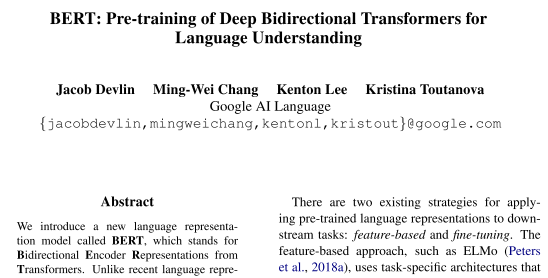
\includegraphics[width=\linewidth]{img/bert-paper01.png}
	\end{column}
\end{columns}

\end{frame}

\begin{frame}{What we won't do}

\begin{columns}
	\begin{column}{0.4\linewidth}
		\begin{figure}
			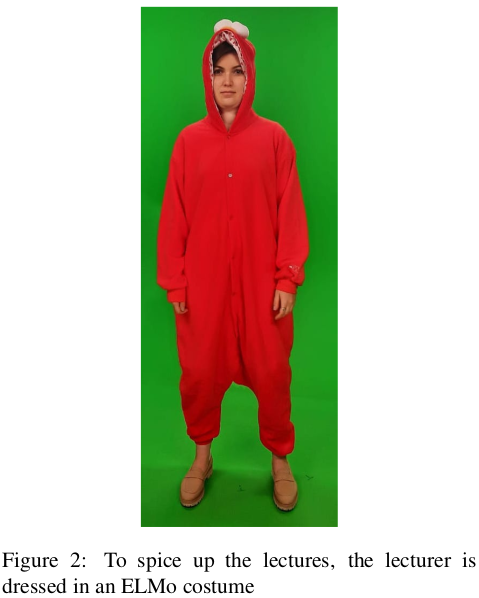
\includegraphics[width=1\linewidth]{img/elmo-workshop-teaching.png}
		\end{figure}
	\end{column}

\begin{column}{0.6\linewidth}
\begin{footnotesize}
\fullcite{artemova-etal-2021-teaching}
\end{footnotesize}

\end{column}
\end{columns}

	
\end{frame}

\section{NLP tasks}

\begin{frame}{Short recap of "NLP tasks"}

Single-sentence "tagging" tasks, such as

-- Part of speech tagging (not in BERT paper)

-- Named Entity Recognition

\begin{figure}
	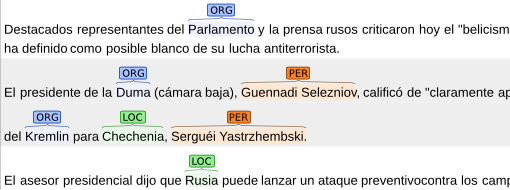
\includegraphics[width=0.7\linewidth]{img/ner.png}
\end{figure}


	
\end{frame}

\begin{frame}{Short recap of "NLP tasks" -- Single sentence}
	
-- Sentiment of a sentence\footnote{\url{https://nlp.stanford.edu/sentiment/treebank.html}}
	
\begin{figure}
	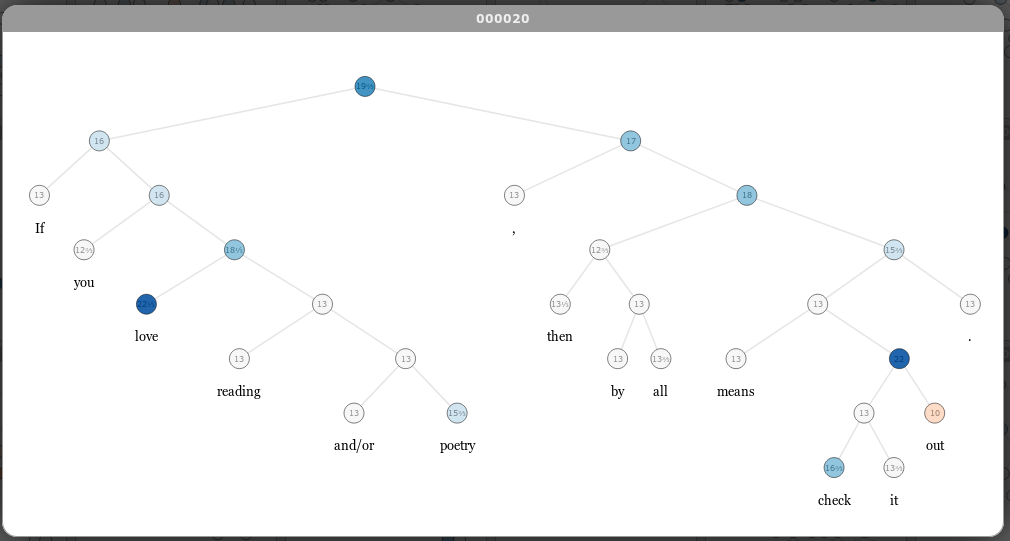
\includegraphics[width=0.95\linewidth]{img/sentiment.png}
\end{figure}

	
\end{frame}

\begin{frame}{More complicated NLP tasks...}
	
Reasoning about two sentences: Natural Language Inference\footnote{\url{https://nlp.stanford.edu/projects/snli/}}

\begin{figure}
	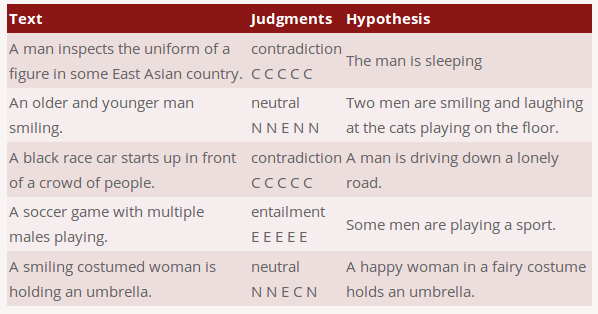
\includegraphics[width=0.9\linewidth]{img/snli.png}
\end{figure}




\end{frame}


\begin{frame}{More complicated NLP tasks...}
	

	Question answering
	
	-- Natural language questions with locations of their answers in Wikipedia articles


	
\end{frame}

\begin{frame}{Why are these NLP tasks hard?}
	
Although some methods can "exploit" artifacts in data,\footnote{\fullcite{Gururangan.et.al.2018.NAACL.short}} the tasks can be truly solved only by

-- Understanding meaning of words (semantics)

-- Understanding relations between meanings

-- Understanding syntax (negations, quantifiers, etc.)

-- Reasoning about the world

	
\end{frame}

\begin{frame}{Roadmap}
	
	\begin{columns}
		
		\begin{column}{0.5\linewidth}
			
			
			NLP tasks $\checkmark$
			
			\begin{itemize}
				\item {\scriptsize Long-range dependencies, hard to represent meaning}
			\end{itemize}
			
			
		\end{column}
		
		\begin{column}{0.5\linewidth}
			

			
		\end{column}
		
	\end{columns}
	
\end{frame}


\section{Deep learning prerequisites}

\begin{frame}{We know the "nail", let's take the hammer}

Prerequisites: We know

\begin{itemize}

	\item  Neural network basics (layers, activations, softmax, convolutions)

	\item  Where are the learnable parameters ("weight matrices" and biases),

	\item  What are loss functions (e.g., cross-entropy for classification)

	\item  How to train them (back-propagation, batches, SGD or Adam)

	\item  Word embeddings (dense semantic representation)

\end{itemize}
	
\end{frame}

\begin{frame}{Roadmap}
	
	\begin{columns}
		
		\begin{column}{0.5\linewidth}
			
			
			NLP tasks $\checkmark$
			
			\begin{itemize}
				\item {\scriptsize Long-range dependencies, hard to represent meaning}
			\end{itemize}
			
			Neural networks $\checkmark$
			
			\begin{itemize}
				\item {\scriptsize Learn non-linear dependencies, learn representations}
			\end{itemize}
			
			Embeddings $\checkmark$
			
			\begin{itemize}
				\item {\scriptsize Dense token representation}
			\end{itemize}
			
			
		\end{column}
		
		\begin{column}{0.5\linewidth}
			
			
		\end{column}
		
	\end{columns}
	
\end{frame}

\section{Neural Machine Translation}

\begin{frame}{Neural machine translation (NMT)}
	Why machine translation here?
	
	BERT builds upon techniques from MT
	
\begin{columns}
	\begin{column}{0.5\textwidth}
	What is machine translation?

\begin{itemize}
	\item Another popular NLP task
	\item Many large-scale parallel corpora available
\end{itemize}

		
	\end{column}
	\begin{column}{0.4\textwidth}
\begin{figure}
	
\includegraphics[width=\linewidth]{img/nmt.jpg}
	\caption{MT is a challenging task!}
\end{figure}	
	
\end{column}
\end{columns}
	
\begin{scriptsize}
Image source: \url{https://languagelog.ldc.upenn.edu/nll/?p=3978}
\end{scriptsize}
\end{frame}

\begin{frame}{Recurrent networks for neural MT}
	
Traditionally \textbf{encoder-decoder} architectures	

\begin{itemize}
	\item One recurrent neural network processes the entire input and generate its dense representation (\textbf{encoder})
	\item Other recurrent network produces one token at the time conditioned on the previous states and generated tokens (\textbf{decoder})
\end{itemize}
\end{frame}


\begin{frame}{Neural MT: Typical architectures (up to 2016-2017)}
		
Long short-term memory (LSTM) / GRU networks


\begin{figure}
	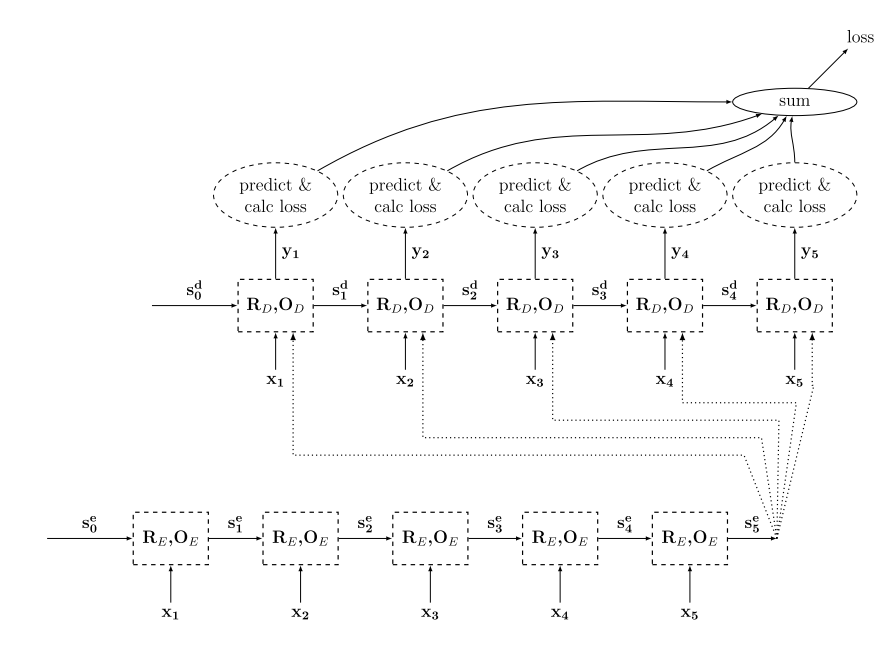
\includegraphics[width=0.65\linewidth]{img/end-dec.png}
	\caption{Encoder-decoder RNN.\footnote{Figure from \citep{Goldberg.2016}}}
\end{figure}
\end{frame}


\begin{frame}{Bottlenecks of RNN for machine translation?}
Inherently \textbf{sequential} nature

\begin{itemize}
	\item No parallelization
	\item Big memory footprint (you must "remember" the entire sequence)
	\item Long-range dependencies modeling: Distance plays a role!
\end{itemize}

...but when the goal is to learn a good representation of the input sequence, why not use...

\begin{itemize}
	\item Convolutional neural networks?
\end{itemize}
	
\end{frame}

\begin{frame}{Convolutional neural nets (CNN) recap}
	
One particular property of CNNs

\begin{itemize}
	\item Modeling dependencies for a \textbf{local context}, but by \textbf{stacking layers}, one exactly controls the context size
\end{itemize}	


\begin{figure}

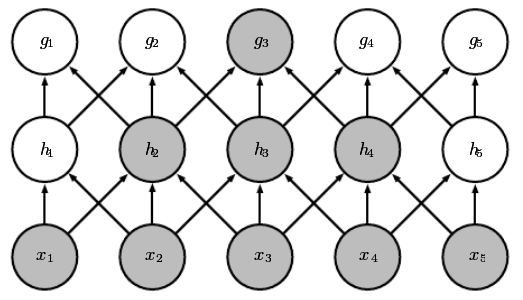
\includegraphics[width=0.5\linewidth]{img/dl-book-cnn.png}	
\caption{Receptive field of units in deeper layers is larger. Source: \fullcite{Goodfellow.et.al.2016.book}}
\end{figure}
\end{frame}


\begin{frame}{Convolutional neural nets for MT}

CNNs competitive with RNNs for MT\footnote{\fullcite{Gehring.et.al.2017a.ICML} (from Facebook AI Research)}

\begin{itemize}
	\item Input tokens as word embeddings (not new) or sub-words (will be explained later)
	\item Fixed-length input? Set-up a maximum length and use \texttt{<PAD>}ding
	\item But positional information of tokens is lost...
\end{itemize}
\end{frame}

\begin{frame}{Convolutional neural nets for MT by \citet{Gehring.et.al.2017a.ICML}}
	
Solution: Positional embeddings
	
\begin{itemize}
	\item For each input position $n$, train another embedding vector $P_n$: $P_1 = (1.12, -78.6, \dots), P_2, \dots, P_N$
	
	\item Word embeddings and position embeddings are simply summed up for each input token
	
	\item Why? The model knows with which part of the input/output is dealing with
	
	\begin{itemize}
		\item Notice: Removing positional embeddings $\to$ only slightly worse performance
	\end{itemize}

	
\end{itemize}


State-of-the-art results and \textbf{9.3--21.3$\times$ faster} than LSTMs on GPU
	
\end{frame}

\begin{frame}{Roadmap}
	
	\begin{columns}
		
		\begin{column}{0.5\linewidth}
			
			
			NLP tasks $\checkmark$
			
			\begin{itemize}
				\item {\scriptsize Long-range dependencies, hard to represent meaning}
			\end{itemize}
			
			Neural networks $\checkmark$
			
			\begin{itemize}
				\item {\scriptsize Learn non-linear dependencies, learn representations}
			\end{itemize}
			
			Embeddings $\checkmark$
			
			\begin{itemize}
				\item {\scriptsize Dense token representation}
			\end{itemize}
			
			Neural machine translation $\checkmark$
			
			\begin{itemize}
				\item {\scriptsize Sequence to sequence models}
				\item {\scriptsize Positional embeddings}
			\end{itemize}
			
		\end{column}
		
		\begin{column}{0.5\linewidth}
			
			
		\end{column}
		
	\end{columns}
	
\end{frame}

\section{Attention ``is all you need"}

\begin{frame}{Attention: Modeling dependencies}
	
Recap: How to model long-range dependencies in input?

\begin{figure}
	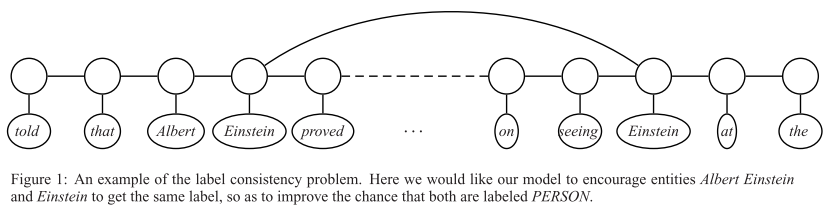
\includegraphics[width=0.95\linewidth]{img/long-deps.png}
\end{figure}


-- RNNs or stacking CNNs

-- \textbf{Self-Attention}: Utilize associations between all input word pairs

\begin{scriptsize}
Figure source: \fullcite{Krishnan.Manning.2006}
\end{scriptsize}

\end{frame}



\begin{frame}{Self-Attention in detail (1)}

	
\begin{figure}
\scalebox{0.75}{\hspace{-2cm}
	\usetikzlibrary{matrix}
\usetikzlibrary{positioning}
\usetikzlibrary{calc}
\usetikzlibrary{backgrounds}
\usetikzlibrary{fit} % for hightligting by calling "fit"

\tikzset{
	mtx/.style={
		matrix of math nodes,
		left delimiter={[}, right delimiter={]}
	},
	hlt/.style={opacity=0.1, line width=4 mm, line cap=round},
	hltr/.style={opacity=0.5, rounded corners=2pt, inner sep=-1pt}
}

\begin{tikzpicture}

\matrix[mtx, ampersand replacement=\&] (X) at (2,2) {
	\mathrm{The} \\ 
	\mathrm{cat}\\ 
	\mathrm{sat}\\ 
	\mathrm{.} \\
	\mathrm{PAD} \\ 
};

\matrix[mtx,  ampersand replacement=\&, right=5ex of X] (matrixh) { 
   \cdots \& h_1 \&  \cdots \\
   \cdots \& h_2 \&  \cdots \\
   \cdots \& h_3 \&  \cdots \\
   \cdots \& h_4 \&  \cdots \\
   \cdots \& h_5 \&  \cdots \\
};

\matrix[mtx, ampersand replacement=\&, nodes={anchor=west}, right=of matrixh] (matrixhtrans) {
   \vdots \& \vdots \&  \vdots \& \vdots \& \vdots \\
   h_1 \& h_2 \& h_3 \& h_4 \& h_5 \\
   \vdots \& \vdots \&  \vdots \& \vdots \& \vdots \\
};

\matrix[mtx, ampersand replacement=\&, nodes={anchor=west}, right=of matrixhtrans] (raw) {
   11 \& 12 \& 13 \& 14 \& 15 \\
   21 \& \ddots \& \& \& \vdots  \\
   31 \&  \& \ddots \&  \& \vdots \\
   41 \&  \&  \& \ddots \& \vdots \\
   51 \&  \cdots \& \cdots  \& \cdots  \& 55 \\
};

%\draw[-stealth, color=red] (X-1-1.south west) -| (beta-6-1.south west);

%\node at ($(X.east) !0.5! (matrixh.west)$) {$*$};
\node at ($(matrixh.east)!0.5!(matrixhtrans.west)$) {$\times$};%
\node at ($(matrixhtrans.east)!0.5!(raw.west)$) {$=$};%


\begin{scope}[on background layer]
%\node[hltr, fill=gray, fit=(beta-1-1)] {};
%\node[hltr, fill=red, fit=(beta-2-1)(beta-3-1)] {};
%\node[hltr, fill=green, fit=(beta-4-1)(beta-6-1)] {};
%\node[hltr, fill=gray, fit=(X-1-1)(X-12-1)] {};
%\node[hltr, fill=orange, fit=(filterg-1-1)(filterg-3-3)] {};
\foreach \in in {1,2,3,4,5} {
\node[hltr, fill=green, fit=(matrixh-\in-1)(matrixh-\in-3)] {};
}
\foreach \in in {1,2,3,4,5} {
\node[hltr, fill=green, fit=(matrixhtrans-1-\in)(matrixhtrans-3-\in)] {};
}
%\node[hltr, fill=orange, fit=(mu-1-1)(mu-1-1)] {};
\node[hltr, fill=lightgray, fit=(raw-1-1)(raw-5-5)] {};
\end{scope}


\foreach \in in {1,2,3,4,5} {
	\draw[->, lightgray, thick] (X-\in-1) to[out = 0, in = 180] (matrixh-\in-1);
}



\begin{scope}[every node/.style={align=center,text width=3cm}]
\node[below=0.2cm of X] (inputdsc) {\scriptsize Input tokens};
\node[below=0.2cm of matrixh] (convdesc) {\scriptsize Matrix $H$ \\ (latent representation)};
\node[below=0.5cm of matrixhtrans] (outdesc) {\scriptsize Matrix $H$ transposed};
\node[below=0.5cm of raw] (outdesc) {\scriptsize Dot product (raw associations) \\  Scale each row by $\sqrt{|h|}$};
%\node[above=0cm of hidden] (hiddendsc) {\scriptsize Hidden layer};
%\node[above=0cm of output] (outputdsc) {\scriptsize Output};


\end{scope}


\end{tikzpicture}
}
\end{figure}
	
\end{frame}

\begin{frame}{Self-Attention in detail (2)}
	
	
	\begin{figure}
		\scalebox{0.75}{\hspace{-2cm}
			\usetikzlibrary{matrix}
\usetikzlibrary{positioning}
\usetikzlibrary{calc}
\usetikzlibrary{backgrounds}
\usetikzlibrary{fit} % for hightligting by calling "fit"

\tikzset{
	mtx/.style={
		matrix of math nodes,
		left delimiter={[}, right delimiter={]}
	},
	hlt/.style={opacity=0.1, line width=4 mm, line cap=round},
	hltr/.style={opacity=0.5, rounded corners=2pt, inner sep=-1pt}
}

\begin{tikzpicture}

\matrix[mtx, ampersand replacement=\&] (X) at (2,2) {
	\mathrm{The} \\ 
	\mathrm{cat}\\ 
	\mathrm{sat}\\ 
	\mathrm{.} \\
	\mathrm{PAD} \\ 
};


\matrix[mtx, ampersand replacement=\&, nodes={anchor=west}, right=of X] (raw) {
   11 \& 12 \& 13 \& 14 \& 15 \\
   21 \& \ddots \& \& \& \vdots  \\
   31 \&  \& \ddots \&  \& \vdots \\
   41 \&  \&  \& \ddots \& \vdots \\
   51 \&  \cdots \& \cdots  \& \cdots  \& 55 \\
};

\matrix[mtx, ampersand replacement=\&, nodes={anchor=west}, right=4cm of raw] (probabilistic) {
   11 \& 12 \& 13 \& 14 \& 15 \\
   21 \& \ddots \& \& \& \dots  \\
   31 \&  \& \ddots \&  \& \dots \\
   41 \&  \&  \& \ddots \& \dots \\
   51 \&  \cdots \& \cdots  \& \cdots  \& 55 \\
};

%\draw[-stealth, color=red] (X-1-1.south west) -| (beta-6-1.south west);

%\node at ($(X.east) !0.5! (matrixh.west)$) {$*$};
%\node at ($(matrixh.east)!0.5!(matrixhtrans.west)$) {$\times$};%
\node at ($(raw.north)!0.5!(probabilistic.north)$) {\scriptsize Softmax (per row)};%


\begin{scope}[on background layer]
%\node[hltr, fill=gray, fit=(beta-1-1)] {};
%\node[hltr, fill=red, fit=(beta-2-1)(beta-3-1)] {};
%\node[hltr, fill=green, fit=(beta-4-1)(beta-6-1)] {};
%\node[hltr, fill=gray, fit=(X-1-1)(X-12-1)] {};
%\node[hltr, fill=orange, fit=(filterg-1-1)(filterg-3-3)] {};

%\node[hltr, fill=orange, fit=(mu-1-1)(mu-1-1)] {};
\node[hltr, fill=lightgray, fit=(raw-1-1)(raw-5-5)] {};
\foreach \in in {1,2,3,4,5} {
	\node[hltr, fill=yellow, fit=(probabilistic-\in-1)(probabilistic-\in-5)] {};
}
\end{scope}


\foreach \in in {1,2,3,4,5} {
	\draw[->, lightgray, thick, dashed] (X-\in-1) to[out = 0, in = 180] (raw-\in-1);
}

\foreach \in in {1,2,3,4,5} {
	\draw[->, lightgray, thick] (raw-\in-5) to[out = 0, in = 180] (probabilistic-\in-1);
}


\begin{scope}[every node/.style={align=center,text width=3cm}]
\node[below=0.2cm of X] (inputdsc) {\scriptsize Input tokens};
\node[below=0cm of raw] (outdesc) {\scriptsize Dot product (raw associations)};
\node[below=0cm of probabilistic] (outdesc) {\scriptsize Normalized associations};
%\node[above=0cm of hidden] (hiddendsc) {\scriptsize Hidden layer};
%\node[above=0cm of output] (outputdsc) {\scriptsize Output};


\end{scope}


\end{tikzpicture}
		}
	\end{figure}
	
	\begin{itemize}
		\item 	Each row corresponds to an input token
		
		\item Each row sums up to 1
		
		\item Each cell shows the "association strength" with all other tokens
		
	\end{itemize}
	
	
\end{frame}



\begin{frame}{Self-Attention in detail (3)}
	
	
	\begin{figure}
		\scalebox{0.75}{\hspace{-2cm}
			\usetikzlibrary{matrix}
\usetikzlibrary{positioning}
\usetikzlibrary{calc}
\usetikzlibrary{backgrounds}
\usetikzlibrary{fit} % for hightligting by calling "fit"

\tikzset{
	mtx/.style={
		matrix of math nodes,
		left delimiter={[}, right delimiter={]}
	},
	hlt/.style={opacity=0.1, line width=4 mm, line cap=round},
	hltr/.style={opacity=0.5, rounded corners=2pt, inner sep=-1pt}
}

\begin{tikzpicture}

\matrix[mtx, ampersand replacement=\&] (X) at (2,2) {
	\mathrm{The} \\ 
	\mathrm{cat}\\ 
	\mathrm{sat}\\ 
	\mathrm{.} \\
	\mathrm{PAD} \\ 
};




\matrix[mtx, ampersand replacement=\&, nodes={anchor=west}, right=of X] (probabilistic) {
   11 \& 12 \& 13 \& 14 \& 15 \\
   21 \& \ddots \& \& \& \dots  \\
   31 \&  \& \ddots \&  \& \dots \\
   41 \&  \&  \& \ddots \& \dots \\
   51 \&  \cdots \& \cdots  \& \cdots  \& 55 \\
};

\matrix[mtx,  ampersand replacement=\&, right=5ex of probabilistic] (matrixh) { 
   \cdots \& h_1 \&  \cdots \\
   \cdots \& h_2 \&  \cdots \\
   \cdots \& h_3 \&  \cdots \\
   \cdots \& h_4 \&  \cdots \\
   \cdots \& h_5 \&  \cdots \\
};

\matrix[mtx,  ampersand replacement=\&, right=5ex of matrixh] (selfattention) { 
   \cdots \& h_1 \&  \cdots \\
   \cdots \& h_2 \&  \cdots \\
   \cdots \& h_3 \&  \cdots \\
   \cdots \& h_4 \&  \cdots \\
   \cdots \& h_5 \&  \cdots \\
};

%\draw[-stealth, color=red] (X-1-1.south west) -| (beta-6-1.south west);

%\node at ($(X.east) !0.5! (matrixh.west)$) {$*$};
\node at ($(probabilistic.east)!0.5!(matrixh.west)$) {$\times$};%
\node at ($(matrixh.east)!0.5!(selfattention.west)$) {$=$};%
%\node at ($(raw.north)!0.5!(probabilistic.north)$) {Softmax (per row)};%


\begin{scope}[on background layer]
%\node[hltr, fill=gray, fit=(beta-1-1)] {};
%\node[hltr, fill=red, fit=(beta-2-1)(beta-3-1)] {};
%\node[hltr, fill=green, fit=(beta-4-1)(beta-6-1)] {};
%\node[hltr, fill=gray, fit=(X-1-1)(X-12-1)] {};
%\node[hltr, fill=orange, fit=(filterg-1-1)(filterg-3-3)] {};

%\node[hltr, fill=orange, fit=(mu-1-1)(mu-1-1)] {};
%\node[hltr, fill=lightgray, fit=(raw-1-1)(raw-5-5)] {};

\foreach \in in {1,2,3,4,5} {
	\node[hltr, fill=green, fit=(matrixh-\in-1)(matrixh-\in-3)] {};
}

\foreach \in in {1,2,3,4,5} {
	\node[hltr, fill=yellow, fit=(probabilistic-\in-1)(probabilistic-\in-5)] {};
}

\foreach \in in {1,2,3,4,5} {
	\node[hltr, fill=orange, fit=(selfattention-\in-1)(selfattention-\in-3)] {};
}
\end{scope}


% \foreach \in in {1,2,3,4,5} {
% 	\draw[->, lightgray, thick, dashed] (X-\in-1) to[out = 0, in = 180] (raw-\in-1);
% }

% \foreach \in in {1,2,3,4,5} {
% 	\draw[->, lightgray, thick] (X-\in-5) to[out = 0, in = 180] (probabilistic-\in-1);
% }

\foreach \in in {1,2,3,4,5} {
	\draw[->, lightgray, thick, dashed] (X-\in-1) to[out = 0, in = 180] (probabilistic-\in-1);
}


\begin{scope}[every node/.style={align=center,text width=3cm}]
\node[below=0.2cm of X] (inputdsc) {\scriptsize Input tokens};
\node[below=0.2cm of matrixh] (convdesc) {\scriptsize Matrix $H$};
% \node[below=0.5cm of raw] (outdesc) {\scriptsize Dot product (raw associations)};
\node[below=0cm of probabilistic] (outdesc) {\scriptsize Normalized associations};
\node[below=0cm of selfattention] (outdesc) {\scriptsize Self-attention};
%\node[above=0cm of hidden] (hiddendsc) {\scriptsize Hidden layer};
%\node[above=0cm of output] (outputdsc) {\scriptsize Output};


\end{scope}


\end{tikzpicture}
		}
	\end{figure}


	Each position in the latent representation of a token is weighted by the association strength with other tokens
	

\end{frame}


\begin{frame}{Self-Attention in detail (4)}
	
	
	\begin{figure}
		\scalebox{0.75}{\hspace{-2cm}
			\usetikzlibrary{matrix}
\usetikzlibrary{positioning}
\usetikzlibrary{calc}
\usetikzlibrary{backgrounds}
\usetikzlibrary{fit} % for hightligting by calling "fit"

\tikzset{
	mtx/.style={
		matrix of math nodes,
		left delimiter={[}, right delimiter={]}
	},
	hlt/.style={opacity=0.1, line width=4 mm, line cap=round},
	hltr/.style={opacity=0.5, rounded corners=2pt, inner sep=-1pt}
}

\begin{tikzpicture}

\matrix[mtx,  ampersand replacement=\& ] (selfattention) at (2,2) { 
   \cdots \& h_1 \&  \cdots \\
   \cdots \& h_2 \&  \cdots \\
   \cdots \& h_3 \&  \cdots \\
   \cdots \& h_4 \&  \cdots \\
   \cdots \& h_5 \&  \cdots \\
};


\matrix[mtx,  ampersand replacement=\&, right=5ex of selfattention] (matrixh) { 
   \cdots \& h_1 \&  \cdots \\
   \cdots \& h_2 \&  \cdots \\
   \cdots \& h_3 \&  \cdots \\
   \cdots \& h_4 \&  \cdots \\
   \cdots \& h_5 \&  \cdots \\
};

\matrix[mtx,  ampersand replacement=\&, right=5ex of matrixh] (residual) { 
   \cdots \& h_1 \&  \cdots \\
   \cdots \& h_2 \&  \cdots \\
   \cdots \& h_3 \&  \cdots \\
   \cdots \& h_4 \&  \cdots \\
   \cdots \& h_5 \&  \cdots \\
};

%\draw[-stealth, color=red] (X-1-1.south west) -| (beta-6-1.south west);

%\node at ($(X.east) !0.5! (matrixh.west)$) {$*$};
% \node at ($(probabilistic.east)!0.5!(matrixh.west)$) {$\times$};%
\node at ($(selfattention.east)!0.5!(matrixh.west)$) {$+$};%
\node at ($(matrixh.east)!0.5!(residual.west)$) {$=$};%
%\node at ($(raw.north)!0.5!(probabilistic.north)$) {Softmax (per row)};%


\begin{scope}[on background layer]
%\node[hltr, fill=gray, fit=(beta-1-1)] {};
%\node[hltr, fill=red, fit=(beta-2-1)(beta-3-1)] {};
%\node[hltr, fill=green, fit=(beta-4-1)(beta-6-1)] {};
%\node[hltr, fill=gray, fit=(X-1-1)(X-12-1)] {};
%\node[hltr, fill=orange, fit=(filterg-1-1)(filterg-3-3)] {};

%\node[hltr, fill=orange, fit=(mu-1-1)(mu-1-1)] {};
%\node[hltr, fill=lightgray, fit=(raw-1-1)(raw-5-5)] {};

\foreach \in in {1,2,3,4,5} {
\node[hltr, fill=green, fit=(matrixh-\in-1)(matrixh-\in-3)] {};
}

\foreach \in in {1,2,3,4,5} {
	\node[hltr, fill=orange, fit=(selfattention-\in-1)(selfattention-\in-3)] {};
}

\foreach \in in {1,2,3,4,5} {
	\node[hltr, fill=blue!20, fit=(residual-\in-1)(residual-\in-3)] {};
}
\end{scope}


% \foreach \in in {1,2,3,4,5} {
% 	\draw[->, lightgray, thick, dashed] (X-\in-1) to[out = 0, in = 180] (raw-\in-1);
% }

% \foreach \in in {1,2,3,4,5} {
% 	\draw[->, lightgray, thick] (X-\in-5) to[out = 0, in = 180] (probabilistic-\in-1);
% }

% \foreach \in in {1,2,3,4,5} {
% 	\draw[->, lightgray, thick, dashed] (X-\in-1) to[out = 0, in = 180] (probabilistic-\in-1);
% }


\begin{scope}[every node/.style={align=center,text width=3cm}]
% \node[below=0.5cm of raw] (outdesc) {\scriptsize Dot product (raw associations)};
\node[below=0cm of matrixh] (convdesc) {\scriptsize Matrix $H$};
\node[below=0cm of selfattention] (outdesc2) {\scriptsize Self-attention};
\node[below=0cm of residual] (outdesc3) {\scriptsize "Residual connections"};
%\node[above=0cm of hidden] (hiddendsc) {\scriptsize Hidden layer};
%\node[above=0cm of output] (outputdsc) {\scriptsize Output};


\end{scope}


\end{tikzpicture}
		}
	\end{figure}
	
\end{frame}



\begin{frame}{Self-Attention in detail: Head}
	
	
	\begin{figure}
		\scalebox{0.75}{\hspace{-1.5cm}
			\usetikzlibrary{matrix}
\usetikzlibrary{positioning}
\usetikzlibrary{calc}
\usetikzlibrary{backgrounds}
\usetikzlibrary{fit} % for hightligting by calling "fit"

\tikzset{
	mtx/.style={
		matrix of math nodes,
		left delimiter={[}, right delimiter={]}
	},
	hlt/.style={opacity=0.1, line width=4 mm, line cap=round},
	hltr/.style={opacity=0.5, rounded corners=2pt, inner sep=-1pt}
}

\begin{tikzpicture}

\matrix[mtx, ampersand replacement=\&] (X) at (0,0) {
	\mathrm{The} \\ 
	\mathrm{cat}\\ 
	\mathrm{sat}\\ 
	\mathrm{.} \\
	\mathrm{PAD} \\ 
};

\matrix[mtx,  ampersand replacement=\&, right=of X ] (selfattention) { 
   \cdots \& h_1 \&  \cdots \\
   \cdots \& h_2 \&  \cdots \\
   \cdots \& h_3 \&  \cdots \\
   \cdots \& h_4 \&  \cdots \\
   \cdots \& h_5 \&  \cdots \\
};


\matrix[mtx,  ampersand replacement=\&, right=5ex of selfattention] (residual) { 
   \cdots \& h_1 \&  \cdots \\
   \cdots \& h_2 \&  \cdots \\
   \cdots \& h_3 \&  \cdots \\
   \cdots \& h_4 \&  \cdots \\
   \cdots \& h_5 \&  \cdots \\
};

\matrix[mtx,  ampersand replacement=\&, right=18ex of residual] (head) { 
   \cdots \& h_1 \&  \cdots \\
   \cdots \& h_2 \&  \cdots \\
   \cdots \& h_3 \&  \cdots \\
   \cdots \& h_4 \&  \cdots \\
   \cdots \& h_5 \&  \cdots \\
};

%\draw[-stealth, color=red] (X-1-1.south west) -| (beta-6-1.south west);

%\node at ($(X.east) !0.5! (matrixh.west)$) {$*$};
% \node at ($(probabilistic.east)!0.5!(matrixh.west)$) {$\times$};%
% \node at ($(selfattention.east)!0.5!(matrixh.west)$) {$+$};%
\node at ($(residual.north)!0.5!(head.north)$) {Further OPs};%




\begin{scope}[on background layer]
%\node[hltr, fill=gray, fit=(beta-1-1)] {};
%\node[hltr, fill=red, fit=(beta-2-1)(beta-3-1)] {};
%\node[hltr, fill=green, fit=(beta-4-1)(beta-6-1)] {};
%\node[hltr, fill=gray, fit=(X-1-1)(X-12-1)] {};
%\node[hltr, fill=orange, fit=(filterg-1-1)(filterg-3-3)] {};

%\node[hltr, fill=orange, fit=(mu-1-1)(mu-1-1)] {};
%\node[hltr, fill=lightgray, fit=(raw-1-1)(raw-5-5)] {};


\foreach \in in {1,2,3,4,5} {
	\node[hltr, fill=orange, fit=(selfattention-\in-1)(selfattention-\in-3)] {};
}

\foreach \in in {1,2,3,4,5} {
	\node[hltr, fill=blue!20, fit=(residual-\in-1)(residual-\in-3)] {};
}

\foreach \in in {1,2,3,4,5} {
	\node[hltr, fill=blue!60, fit=(head-\in-1)(head-\in-3)] {};
}

\end{scope}


% \foreach \in in {1,2,3,4,5} {
% 	\draw[->, lightgray, thick, dashed] (X-\in-1) to[out = 0, in = 180] (raw-\in-1);
% }

% \foreach \in in {1,2,3,4,5} {
% 	\draw[->, lightgray, thick] (X-\in-5) to[out = 0, in = 180] (probabilistic-\in-1);
% }

% \foreach \in in {1,2,3,4,5} {
% 	\draw[->, lightgray, thick, dashed] (X-\in-1) to[out = 0, in = 180] (probabilistic-\in-1);
% }

\foreach \in in {1,2,3,4,5} {
	\draw[->, lightgray, thick, dashed] (X-\in-1) to[out = 0, in = 180] (selfattention-\in-1);
}

\foreach \in in {1,2,3,4,5} {
	\draw[->, lightgray, thick, dashed] (selfattention-\in-3) to[out = 0, in = 180] (residual-\in-1);
}

\foreach \in in {1,2,3,4,5} {
	\draw[->, lightgray, thick, dashed] (residual-\in-3) to[out = 0, in = 180] (head-\in-1);
}

\begin{scope}[every node/.style={align=center,text width=3cm}]
% \node[below=0.5cm of raw] (outdesc) {\scriptsize Dot product (raw associations)};
\node[below=0cm of selfattention] (outdesc2) {\scriptsize Self-attention};
\node[below=0cm of residual] (outdesc3) {\scriptsize "Residual connections"};
\node[below=0cm of head] (outdesc3) {\scriptsize Attention "head" output};
%\node[above=0cm of hidden] (hiddendsc) {\scriptsize Hidden layer};
%\node[above=0cm of output] (outputdsc) {\scriptsize Output};


\end{scope}


\end{tikzpicture}
		}
	\end{figure}
	
	Further operations
	
	\begin{itemize}
		\item Layer normalization
		\item Feed-forward layer with ReLU
		\item Another residual connection and layer normalization
	\end{itemize}
	
\end{frame}


\begin{frame}{Self-attention: More subtleties}
	
	\begin{itemize}
		\item Run N attention "heads" in parallel and concatenate
		\item Stack on top of each other M-times
	\end{itemize}
	
	
	Why self-attention?
	
	\begin{itemize}
		\item Self-attention layer connects all positions with a constant number of sequentially executed operations
		\item Recurrent layer requires O(n) sequential operations
		\item Self-attention layers are \textbf{fast}
	\end{itemize}
	
	\begin{footnotesize}
	\fullcite{Vaswani.et.al.2017}
	\end{footnotesize}

	
\end{frame}



\begin{frame}{Roadmap}
	
	\begin{columns}
		
		\begin{column}{0.5\linewidth}
			
			
			NLP tasks $\checkmark$
			
			\begin{itemize}
				\item {\scriptsize Long-range dependencies, hard to represent meaning}
			\end{itemize}
			
			Neural networks $\checkmark$
			
			\begin{itemize}
				\item {\scriptsize Learn non-linear dependencies, learn representations}
			\end{itemize}
			
			Embeddings $\checkmark$
			
			\begin{itemize}
				\item {\scriptsize Dense token representation}
			\end{itemize}
			
			Neural machine translation $\checkmark$
			
			\begin{itemize}
				\item {\scriptsize Sequence to sequence models}
				\item {\scriptsize Positional embeddings}
			\end{itemize}
			
		\end{column}
		
		\begin{column}{0.5\linewidth}
			
			Attention $\checkmark$
			
			\begin{itemize}
				\item {\scriptsize Efficient long-range dependencies}
			\end{itemize}
			
		
			
		\end{column}
		
	\end{columns}
	
\end{frame}


\section{Out-of-vocabulary words}

\begin{frame}{Pitfalls of machine translation: Vocabulary and Out-of-vocabulary (OOV)}

\begin{itemize}
	\item MT often with fixed word vocabularies
	\begin{itemize}
		\item Even though translation is fundamentally an open vocabulary problem (names, numbers, dates etc.).
		\item Initially, the most frequent words were used, and all others \texttt{<UNK>}\footnote{\fullcite{Koehn.2017}}
	\end{itemize}
	\item Translation of out-of-vocabulary (OOV) words
	\begin{itemize}
		\item 	Rare words (OOV) handled with a back-off dictionary, or simply copied 1:1 from source to target
	\end{itemize}

	
\end{itemize}

\end{frame}


\begin{frame}{Sub-word units: Motivation?}
	
Sub-words for voice search (Japanese, Korean)\footnote{\fullcite{Schuster.Nakajima.2012}}

\begin{itemize}
	\item Too large vocabularies for these two languages would produce way too many OOVs
\end{itemize}

Later known as WordPiece model

\begin{itemize}
	\item Adapted by Google's Neural Machine Translation\footnote{\fullcite{Wu.et.al.2016.GoogleMT}} and eventually by BERT
\end{itemize}


\end{frame}

\begin{frame}{Sub-word units: Motivation?}
	

But why should sub-word units give better translations than copying or back-off dictionary?
	
-- Open-vocabulary MT better by representing rare and unseen words as a sequence of subword units\footnote{\fullcite{Sennrich.et.al.2016.ACL}}
	
	
\end{frame}


\begin{frame}{What are WordPiece units?}

\begin{itemize}
	\item Similar to a vocabulary: A list of all known (sub-)words, including characters
	\begin{itemize}
		\item Each word is either entirely a WordPiece unit, or can be split into several WordPiece units
	\end{itemize}
	\item Splitting a text into the trained WordPiece model shipped along with BERT:
\end{itemize}

\begin{small}
\texttt{tokenizer.tokenize("All human beings are born free and equal in dignity and rights.")}
\\
\texttt{['all', 'human', 'beings', 'are', 'born', 'free', 'and', 'equal', 'in', 'dignity', 'and', 'rights', '.']}
\end{small}

	
\end{frame}






\begin{frame}{WordPiece units: Multilingual}
	
\begin{figure}
	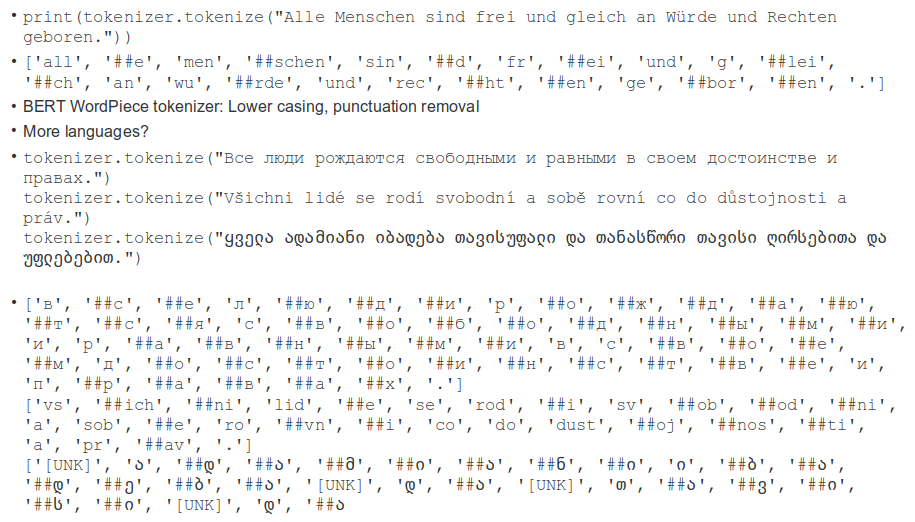
\includegraphics[width=\linewidth]{img/word-piece.png}
\end{figure}
	
\end{frame}





\begin{frame}{Training WordPiece inventory}
	
	\begin{enumerate}
		\item Init the WordPiece inventory with all characters (in all alphabets)
		\item For each possible tuple of known WordPieces
		\begin{itemize}
			\item Create a new candidate WordPiece from the tuple (simply concatenate)
			\item Build a language model and compute likelihood on the corpus
		\end{itemize}
		\item Select the candidate with the maximum likelihood increase and add to the WordPiece inventory; Go back to 2 or finish, if WordPiece inventory has the desired size
	\end{enumerate}
	
	
	\bigskip
	
	\scriptsize{\fullcite{Schuster.Nakajima.2012}}
	
\end{frame}



\begin{frame}{Roadmap}
	
	\begin{columns}
		
		\begin{column}{0.5\linewidth}
			
			
			NLP tasks $\checkmark$
			
			\begin{itemize}
				\item {\scriptsize Long-range dependencies, hard to represent meaning}
			\end{itemize}
			
			Neural networks $\checkmark$
			
			\begin{itemize}
				\item {\scriptsize Learn non-linear dependencies, learn representations}
			\end{itemize}
			
			Embeddings $\checkmark$
			
			\begin{itemize}
				\item {\scriptsize Dense token representation}
			\end{itemize}
			
			Neural machine translation $\checkmark$
			
			\begin{itemize}
				\item {\scriptsize Sequence to sequence models}
				\item {\scriptsize Positional embeddings}
			\end{itemize}
			
		\end{column}
		
		\begin{column}{0.5\linewidth}
			
			Attention $\checkmark$
			
			\begin{itemize}
				\item {\scriptsize Efficient long-range dependencies}
			\end{itemize}
			
			
			Out-of-vocabulary words $\checkmark$
			
			\begin{itemize}
				\item {\scriptsize WordPiece sub-word units can be truly multi-lingual and prevent OOV}
			\end{itemize}
			
			
			
		\end{column}
		
	\end{columns}
	
\end{frame}


\section{Multi-task learning}


\begin{frame}{Multi-task Learning}

\begin{columns}
\begin{column}{0.5\linewidth}
Approach to inductive transfer that improves generalization

\bigskip	

By learning tasks in parallel while using a shared representation
	
\end{column}
\begin{column}{0.5\linewidth}
\begin{figure}
	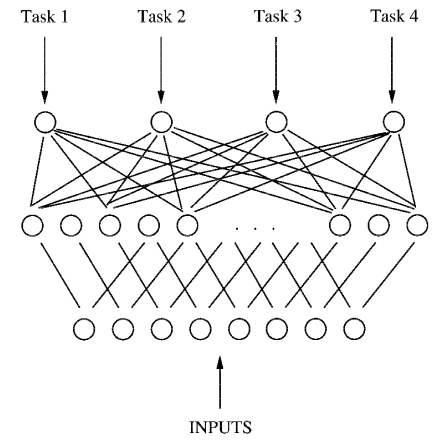
\includegraphics[width=\linewidth]{img/multitask.png}	
\end{figure}
	
\end{column}
\end{columns}
	
\bigskip

\begin{footnotesize}
	\fullcite{Caruana.1997}
\end{footnotesize}
	
	
\end{frame}



\begin{frame}{Multi-task learning in NLP}
	
	\begin{columns}
		\begin{column}{0.5\linewidth}
			
			\begin{small}
			\emph{"In case we suspect the existence of a hierarchy between the different tasks, we show that it is worth-while to incorporate this knowledge in the MTL architecture’s design, by making lower level tasks affect the lower levels of the representation." }
			\end{small}			
		\end{column}
	\begin{column}{0.5\linewidth}
		
		\begin{figure}
			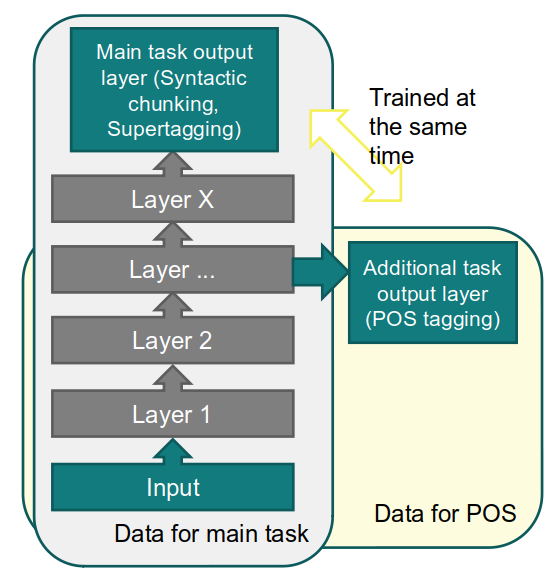
\includegraphics[width=\linewidth]{img/multitask-nlp.png}
		\end{figure}
	\end{column}
	\end{columns}

\bigskip

\begin{footnotesize}
	\fullcite{Sogaard.Goldberg.2016}
\end{footnotesize}

\end{frame}


\begin{frame}{Learn a sentence representation on a different task}
	
\begin{figure}
	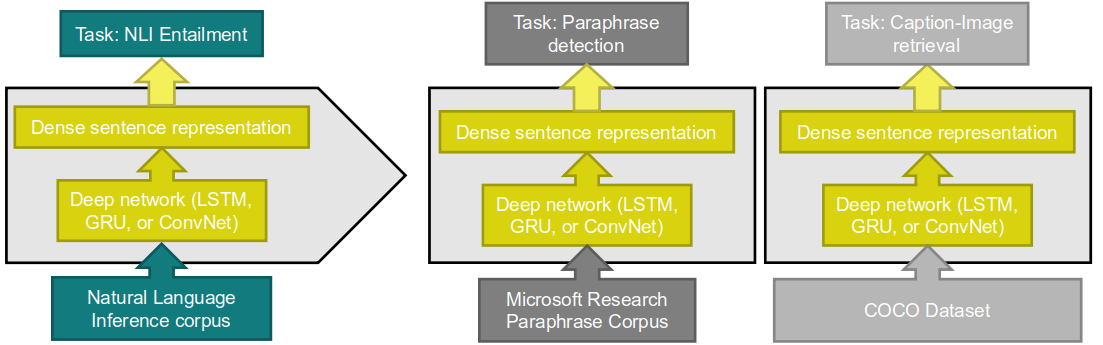
\includegraphics[width=0.9\linewidth]{img/transfer.png}
\end{figure}

\begin{small}
\emph{"Models learned on NLI can perform better than models trained in unsupervised conditions or on other supervised tasks."}\footnote{\fullcite{Conneau.et.al.2017.EMNLP}}
\end{small}

	
\end{frame}


\begin{frame}{Roadmap}
	
	\begin{columns}
		
		\begin{column}{0.5\linewidth}
			
			
			NLP tasks $\checkmark$
			
			\begin{itemize}
				\item {\scriptsize Long-range dependencies, hard to represent meaning}
			\end{itemize}
			
			Neural networks $\checkmark$
			
			\begin{itemize}
				\item {\scriptsize Learn non-linear dependencies, learn representations}
			\end{itemize}
			
			Embeddings $\checkmark$
			
			\begin{itemize}
				\item {\scriptsize Dense token representation}
			\end{itemize}
			
			Neural machine translation $\checkmark$
			
			\begin{itemize}
				\item {\scriptsize Sequence to sequence models}
				\item {\scriptsize Positional embeddings}
			\end{itemize}
			
		\end{column}
		
		\begin{column}{0.5\linewidth}
			
			Attention $\checkmark$
			
			\begin{itemize}
				\item {\scriptsize Efficient long-range dependencies}
			\end{itemize}
			
			
			Out-of-vocabulary words $\checkmark$
			
			\begin{itemize}
				\item {\scriptsize WordPiece sub-word units can be truly multi-lingual and prevent OOV}
			\end{itemize}
			
			
			Multi-task learning $\checkmark$
			
			\begin{itemize}
				\item {\scriptsize Shared representation improves generalization; transfer learning}
			\end{itemize}
			
		
		\end{column}
		
	\end{columns}
	
\end{frame}

\section{``Unsupervised'' Pre-Training}

\begin{frame}{"Un-supervised" Pre-Training}

\begin{itemize}
	\item Deep neural nets are trained with full supervision
	\begin{itemize}
		\item Even autoencoders are supervised by the reconstruction error
	\end{itemize}
	\item "Unsupervised" training scenario usually means:
	\begin{itemize}
		\item 	I don't have any labeled data for my target task (e.g., no labels for "word similarity")
		\item 	But I can design a proxy supervised task (e.g., "given a context of a missing word, predict that word")
		\item	And create positive and negative instances by exploiting a large unlabeled corpus (e.g., words in their context as positive, and randomly swapped words with their context as negative)
	\end{itemize}
\end{itemize}


\end{frame}

\begin{frame}{Roadmap}
	
	\begin{columns}
		
		\begin{column}{0.5\linewidth}
			
			
			NLP tasks $\checkmark$
			
			\begin{itemize}
				\item {\scriptsize Long-range dependencies, hard to represent meaning}
			\end{itemize}
			
			Neural networks $\checkmark$
			
			\begin{itemize}
				\item {\scriptsize Learn non-linear dependencies, learn representations}
			\end{itemize}
			
			Embeddings $\checkmark$
			
			\begin{itemize}
				\item {\scriptsize Dense token representation}
			\end{itemize}
			
			Neural machine translation $\checkmark$
			
			\begin{itemize}
				\item {\scriptsize Sequence to sequence models}
				\item {\scriptsize Positional embeddings}
			\end{itemize}
			
		\end{column}
		
		\begin{column}{0.5\linewidth}
			
			Attention $\checkmark$
			
			\begin{itemize}
				\item {\scriptsize Efficient long-range dependencies}
			\end{itemize}
			
			
			Out-of-vocabulary words $\checkmark$
			
			\begin{itemize}
				\item {\scriptsize WordPiece sub-word units can be truly multi-lingual and prevent OOV}
			\end{itemize}
			
			
			Multi-task learning $\checkmark$
			
			\begin{itemize}
				\item {\scriptsize Shared representation improves generalization; transfer learning}
			\end{itemize}
			
			"Unsupervised" Pre-Training $\checkmark$
			
			\begin{itemize}
				\item {\scriptsize Proxy task and unlimited data from unlabeled corpora}
			\end{itemize}
			
		\end{column}
		
	\end{columns}
	
\end{frame}


\section{BERT}


\begin{frame}{BERT: Very abstract view}
	
\begin{figure}
	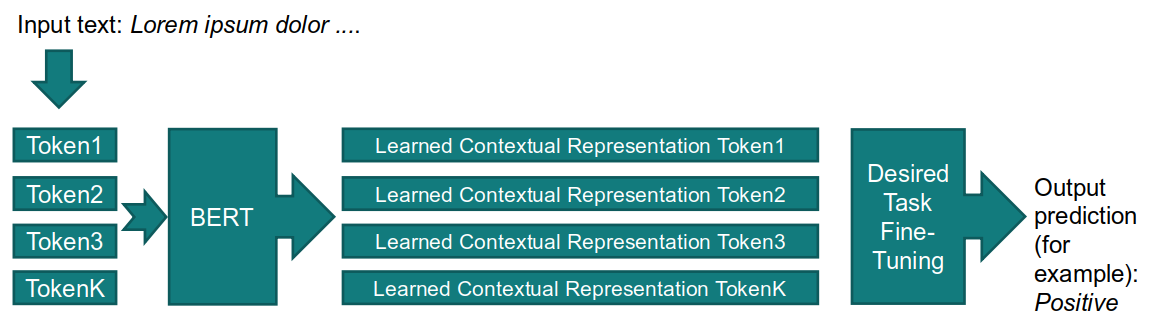
\includegraphics[width=\linewidth]{img/bert1.png}
\end{figure}	
	
\end{frame}


\begin{frame}{BERT: Tokenization}
	
Tokenizing into a multilingual WordPiece inventory

\begin{itemize}
	\item Recall that WordPiece units are sub-word units
	\item 30,000 WordPiece units (newer models 110k units, 100 languages)
\end{itemize}

Implications: BERT can "consume" any language

	
\end{frame}


\begin{frame}{BERT: Input representation}
	
\begin{itemize}
	\item Each WordPiece token from the input is represented by a \textbf{WordPiece embedding} (randomly initialized)
	\item Each position from the input is associated with a \textbf{positional embedding} (also randomly initialized)
	\item Input length limited to \textbf{512} WordPiece tokens, using \texttt{<PAD>}ding
	\item Special tokens
	\begin{itemize}
		\item The fist token is always a special token \textbf{[CLS]}
		\item If the task involves two sentences (e.g., NLI), these two sentences are separated by a special token \textbf{[SEP]}; also special two \textbf{segment position embeddings} 
	\end{itemize}

\end{itemize}
	
\end{frame}


\begin{frame}{BERT: Input representation summary}
	
\begin{figure}
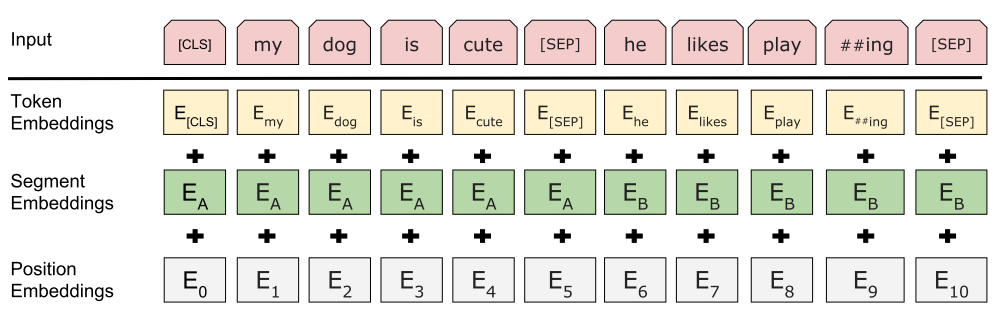
\includegraphics[width=\linewidth]{img/bert-input.png}	
\end{figure}
	
\end{frame}

\begin{frame}{BERT: Very abstract view}
	
	\begin{figure}
		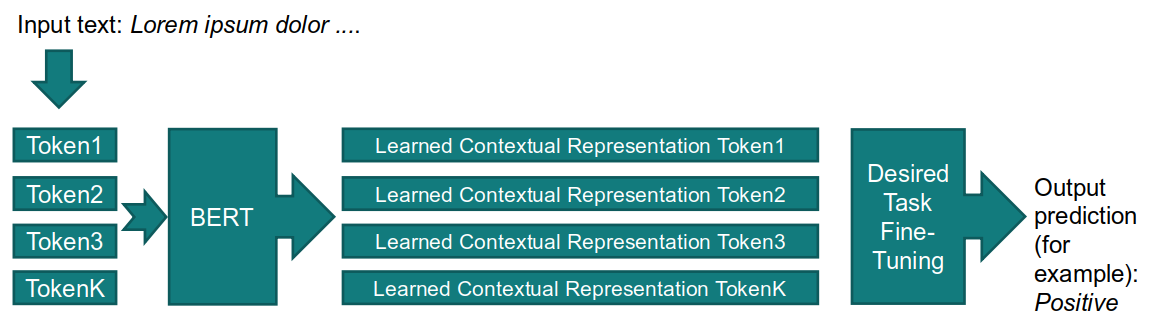
\includegraphics[width=\linewidth]{img/bert1.png}
	\end{figure}	
	
\end{frame}

\begin{frame}{BERT: The Transformer}
	
	\begin{columns}
		\begin{column}{0.6\linewidth}
			\begin{itemize}
				\item The good-old-friend "Self-Attention"
				\item Multiple parallel attention "heads” (16 heads)
				\item With residual connections
				\item With layer normalization
				\item Stacked on top of each other (24-times)
				\item 310,000,000 trainable parameters
				\item ...we've seen that already
			\end{itemize}
		\end{column}
		\begin{column}{0.3\linewidth}
			\begin{figure}
			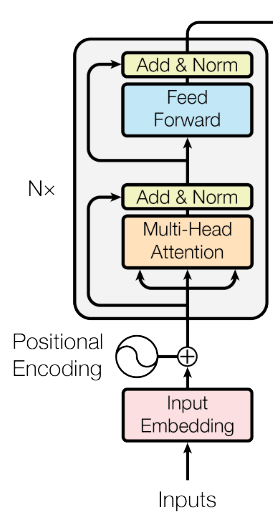
\includegraphics[width=\linewidth]{img/transformer.png}
			\end{figure}
		\end{column}
	\end{columns}
	
\end{frame}

\begin{frame}{BERT: Very abstract view}
	
	\begin{figure}
		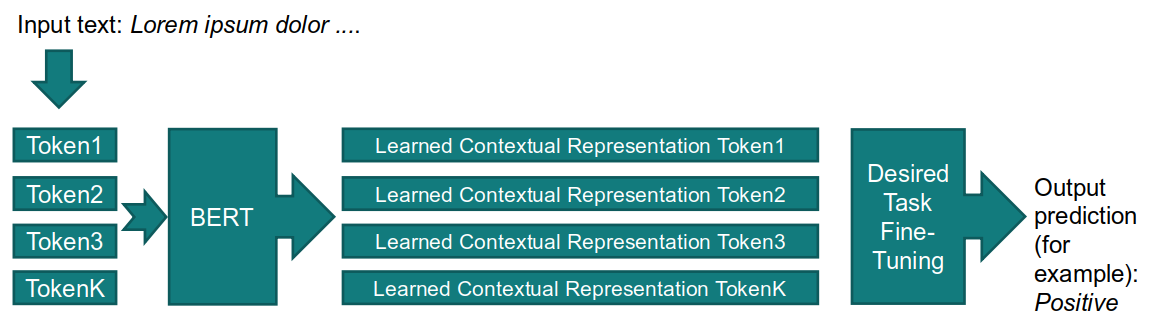
\includegraphics[width=\linewidth]{img/bert1.png}
	\end{figure}	
	
\end{frame}


\begin{frame}{BERT: Representing various NLP tasks}
	
\begin{figure}
	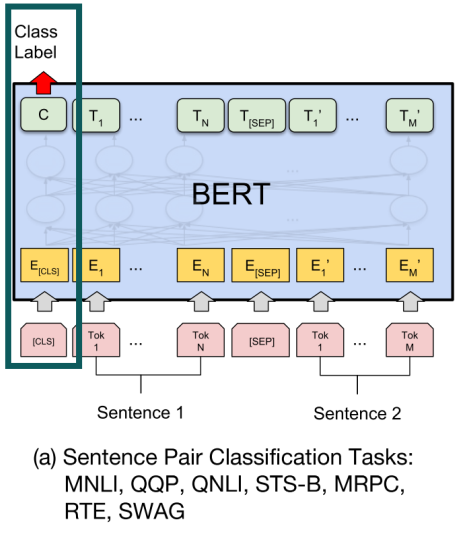
\includegraphics[width=0.5\linewidth]{img/task1.png}
\end{figure}
	
That explains the special [CLS] token at sequence start
	
\end{frame}



\begin{frame}{BERT: Representing various NLP tasks}
	
	\begin{figure}
		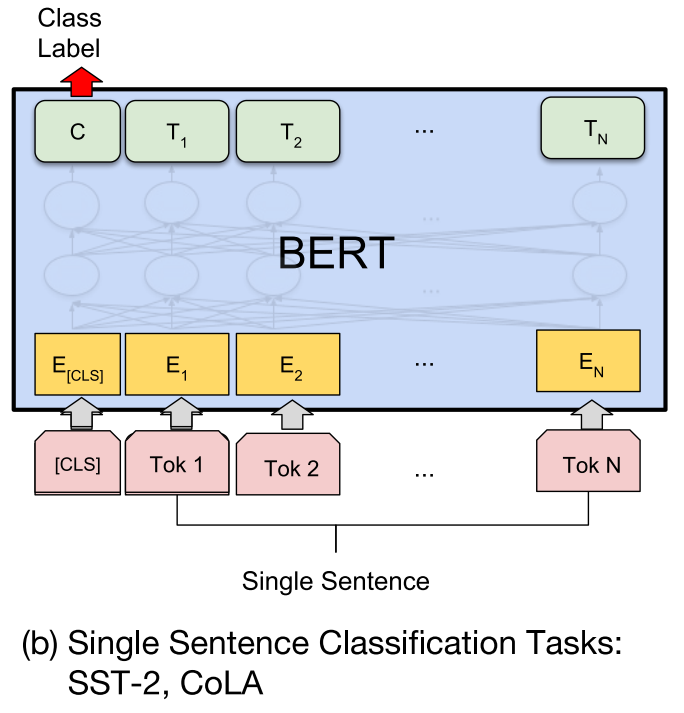
\includegraphics[width=0.6\linewidth]{img/task2.png}
	\end{figure}
	
	
\end{frame}



\begin{frame}{BERT: Representing various NLP tasks}
	
	\begin{figure}
		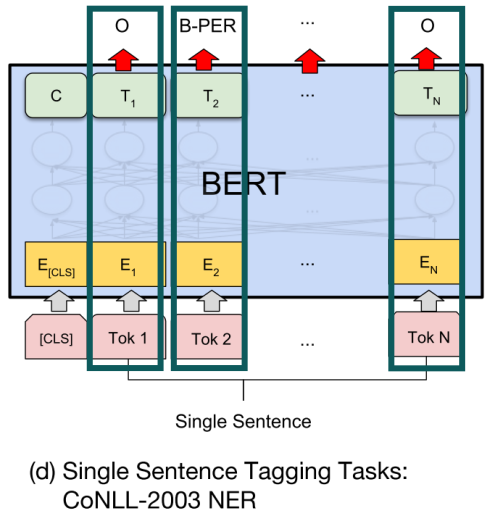
\includegraphics[width=0.5\linewidth]{img/task3.png}
	\end{figure}


Not conditioned on surrounding predictions	

\end{frame}

\begin{frame}{BERT: Very abstract view}
	
	\begin{figure}
		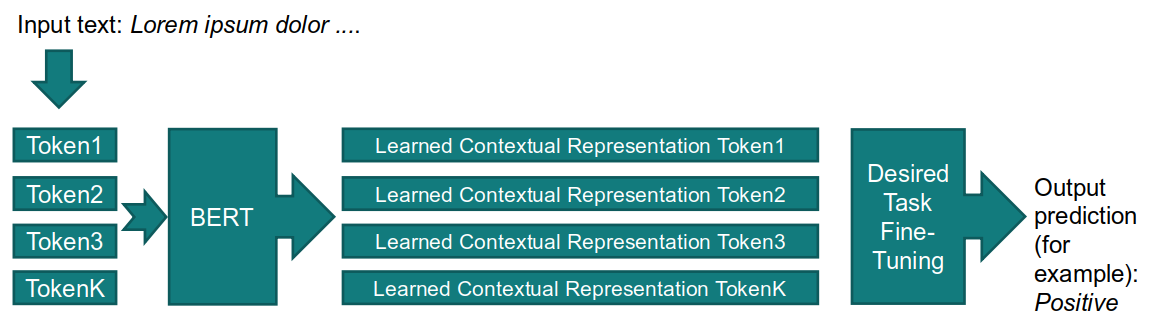
\includegraphics[width=\linewidth]{img/bert1.png}
	\end{figure}	
	
\end{frame}


\begin{frame}{BERT: "Unsupervised" multi-task pre-training}

Prepare two auxiliary tasks that need no labeled data

\bigskip

\begin{columns}
	\begin{column}{0.5\linewidth}
		\begin{small}
			Task 1: Cloze-test task
			\begin{itemize}
				\item 	Predict the masked WordPiece unit (multi-class, 30k classes)
			\end{itemize}


		Task 2: Consecutive segment prediction

			\begin{itemize}
				\item Did the second text segment appeared after the first segment? (binary)
			\end{itemize}
		\end{small}
		
	\end{column}
	\begin{column}{0.5\linewidth}
		
		\begin{figure}
			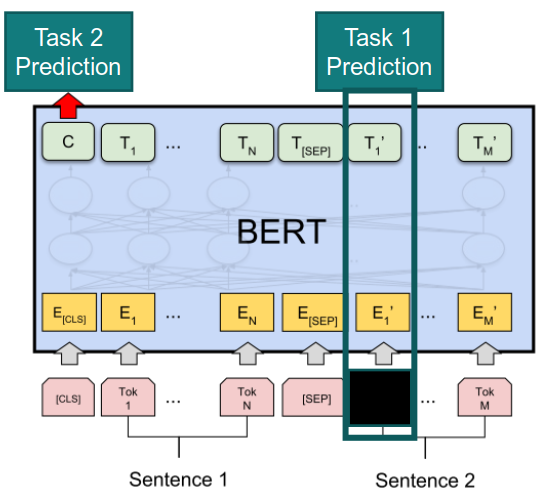
\includegraphics[width=\linewidth]{img/bert-pretraining.png}
		\end{figure}
	\end{column}
	
\end{columns}
\end{frame}




\begin{frame}{BERT: Pre-training data generation}

Take the entire Wikipedia (in 100 languages; 2,5 billion words)

To generate a single training instance, sample two segments (max combined length 512 WordPiece tokens)

\begin{itemize}
	\item For Task 2, replace the second segment randomly in 50\% (negative samples)
	\item For Task 1, choose random 15\% of the tokens, and in 80\% replace with a [MASK] 
\end{itemize}
	

\end{frame}


\begin{frame}{BERT: Pre-training data -- Simplified example}
	
\begin{columns}
	\begin{column}{0.5\linewidth}
		\begin{figure}
			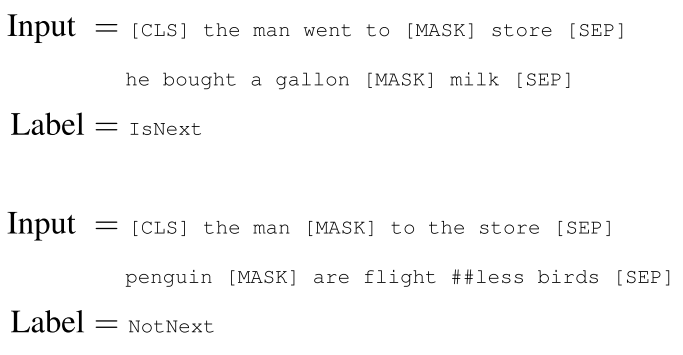
\includegraphics[width=\linewidth]{img/bert-pretraining2.png}
		\end{figure}
	\end{column}
	\begin{column}{0.5\linewidth}
	\begin{small}

	\begin{itemize}
		\item $<$PAD$>$ding is missing
		\item The actual segments are longer and not necessarily actual sentences (just spans)
		\item The WordPiece tokens match full words / morphology well in this English text, but recall the ones we have seen before
	\end{itemize}
	\end{small}
	\end{column}
\end{columns}
	
	
\end{frame}




\begin{frame}{BERT: Very abstract view}
	
	\begin{figure}
		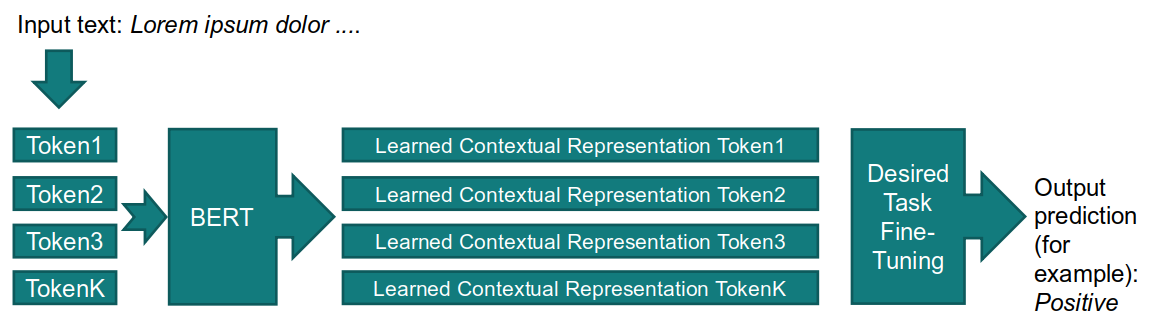
\includegraphics[width=\linewidth]{img/bert1.png}
	\end{figure}	

Pretraining this monster took them 4 days on 64 TPU chips
(estimated \$500 USD)

\bigskip

Once pre-trained, transfer and "fine-tune" on your small-data task and get state-of-the-art results :)


\end{frame}





\begin{frame}{Roadmap}

\begin{columns}
	
\begin{column}{0.5\linewidth}
	
	
NLP tasks $\checkmark$

\begin{itemize}
	\item {\scriptsize Long-range dependencies, hard to represent meaning}
\end{itemize}

Neural networks $\checkmark$

\begin{itemize}
	\item {\scriptsize Learn non-linear dependencies, learn representations}
\end{itemize}

Embeddings $\checkmark$

\begin{itemize}
	\item {\scriptsize Dense token representation}
\end{itemize}

Neural machine translation $\checkmark$

\begin{itemize}
	\item {\scriptsize Sequence to sequence models}
	\item {\scriptsize Positional embeddings}
\end{itemize}

\end{column}

\begin{column}{0.5\linewidth}

Attention $\checkmark$

\begin{itemize}
	\item {\scriptsize Efficient long-range dependencies}
\end{itemize}


Out-of-vocabulary words $\checkmark$

\begin{itemize}
	\item {\scriptsize WordPiece sub-word units can be truly multi-lingual and prevent OOV}
\end{itemize}


Multi-task learning $\checkmark$

\begin{itemize}
	\item {\scriptsize Shared representation improves generalization; transfer learning}
\end{itemize}

"Unsupervised" Pre-Training $\checkmark$

\begin{itemize}
	\item {\scriptsize Proxy task and unlimited data from unlabeled corpora}
\end{itemize}

\end{column}

\end{columns}

\end{frame}


\begin{frame}{BERT Recap}
	
	BERT stays on the shoulders of many clever concepts and techniques, mastered into a single model
	
\end{frame}

\section{What do we know about how BERT works?}

\begin{frame}{Highly recommended reading}
	
	\emph{``BERTology has clearly come a long way, but it is fair to say we still have more questions than answers about how BERT works.''}
	
	\bigskip
	
	\fullcite{Rogers.et.al.2020.BERT}
	
\end{frame}


\begin{frame}{License and credits}
	
	\begin{columns}
		\begin{column}{0.7\textwidth}
			Licensed under Creative Commons Attribution-ShareAlike 4.0 International (CC BY-SA 4.0)
		\end{column}
		\begin{column}{0.2\textwidth}
			
\includegraphics[width=0.9\linewidth]{img/cc-by-sa-icon.pdf}
		\end{column}
	\end{columns}
	
	\bigskip
	
	Credits
	
	\begin{scriptsize}
		
		Ivan Habernal
		
		Content from ACL Anthology papers licensed under CC-BY \url{https://www.aclweb.org/anthology}
		
	
	\end{scriptsize}
	
\end{frame}

\begin{frame}[allowframebreaks]{References}
	\printbibliography
	%  \bibliography{bibliography}
	%  \bibliographystyle{abbrv}
\end{frame}



\end{document}

